% !TEX encoding = UTF-8 Unicode
\documentclass[a4paper,12pt]{article}

%-----------------------------------------Include package & set up some thing-----------------------------------------------
\usepackage{fontspec}
\setmainfont{Times New Roman} %set font
\usepackage{enumitem} % to format list
\usepackage{amsmath}
\usepackage{listings} % quote code
\usepackage{color}
\usepackage{hyperref} % cite hyperlink & bookmarks
\usepackage{setspace} % space
\usepackage{graphicx} % insert image
\usepackage{subcaption} % Multiple images
\usepackage{float}
\usepackage[margin=1in, footskip = 0.25in]{geometry} % Change margin with geometry package

\hypersetup{unicode, colorlinks,linkcolor=black, urlcolor=cyan} % format hyperlink and bookmarks

%Define title
\title{Báo cáo bài tập 7}
\author{1612174 - Phùng Tiến Hào - \href{mailto:tienhaophung@gmail.com}{tienhaophung@gmail.com}}
\date{12/05/2019}

%Code formatting with the listing package
\definecolor{codegreen}{rgb}{0,0.6,0}
\definecolor{codegray}{rgb}{0.3,0.3,0.3}
\definecolor{codepurple}{rgb}{0.58,0,0.82}
\definecolor{backcolour}{rgb}{0.92,0.92,0.88}

\lstdefinestyle{mystyle}{
	backgroundcolor=\color{backcolour},   
	commentstyle=\color{codegreen},
	keywordstyle=\color{blue},
	numberstyle=\tiny\color{codegray},
	stringstyle=\color{codepurple},
	basicstyle=\footnotesize,
	breakatwhitespace=false,         
	breaklines=true,                 
	captionpos=b,                    
	keepspaces=true,                 
	numbers=left,                    
	numbersep=5pt,                  
	showspaces=false,                
	showstringspaces=false,
	showtabs=false,                  
	tabsize=2,
	columns=fullflexible,
	frame=single
}

\lstset{style=mystyle}

\begin{document}
	\pagenumbering{gobble}
	\maketitle
	\newpage
	
	\doublespacing
	\tableofcontents
	\singlespace
	
	\newpage
	\pagenumbering{arabic}
	
	\textbf{Dữ liệu khảo sát:} SpeedDating trong package Lock5withR\\
	
	Load package và thêm các thư viện cần thiết trước khi đi vào xử lý:
	\begin{lstlisting}[language=R]
	require(Lock5withR) # Load package
	library(Lock5withR)
	library(mosaic)
	
	# head(SpeedDating)
	attach(SpeedDating) # Avoid dollar sign before each varibles name
	\end{lstlisting}
	
	\section{Chi-square Goodness of Fit Test for single catogorical variable}
	\subsection{DecisionMale (Yes/No)}
	
	Giả sử, ta cần khảo sát tỉ lệ nam phản hồi (Yes/No) cho quần thể (population) là toàn bộ học sinh nam của trường Columbia. Từ tổng thể, ta thu thập được một mẫu dữ liệu ngẫu nhiên (random sample) gồm 276 quan sát trong đó có 146 phản hồi "Yes" và 130 phản hồi "No". Dựa vào mẫu dữ liệu này, ta kiểm định nghi vấn "tỉ lệ phản hồi Yes và phản hồi No bằng nhau" với mức ý nghĩa (significance level) 5\%.
	
	Tỉ lệ kỳ vọng (Expected proportion) là $0.5$ cho các phản hồi "Yes" và "No".
	
	Ta thực hiện kiểm định giả thuyết:
	
	\begin{equation*}
		\begin{cases}
		H_0: p_{Yes} = p_{No} = 0.5\\
		H_1: p_{Yes} \neq p_{No}
		\end{cases}
	\end{equation*}
	với mức ý nghĩa $\alpha = 0.5\%$
	
	Lưu ý: Để dùng Chi-square để kiểm định thì các ô quan sát phải ít nhất 5.
	
	\begin{lstlisting}[language=R]
	> # Load data
	> data <- DecisionMale
	> # Significant level
	> alpha <- 0.05
	> # Frequency table
	> t <- table(data); t
	data
	No Yes 
	130 146 
	> # Chisq test
	> res <- chisq.test(t); res
	
	Chi-squared test for given probabilities
	
	data:  t
	X-squared = 0.92754, df = 1, p-value = 0.3355
	
	> # If p.value < alpha, we ignore H0
	> (res$p.value < alpha)
	[1] FALSE
	> # Expected values
	> res$expected
	No Yes 
	138 138
	\end{lstlisting}
	
	Vì $p-value > \alpha$ nên ta không bác bỏ $H_0$. Như vậy, với mức ý nghĩa 5\%, ta không có đủ căn cứ để bác bỏ "tỉ lệ phản hồi "Yes" bằng "No"".\\
	
	\textbf{Nhận xét:}\\
	\begin{itemize}
		\item Ta thấy rằng expected values và observed values chênh lệch không nhiều, do đó không đóng góp nhiều vào $\mathcal{X}^2$.
	\end{itemize}
	
	
	
	\subsection{RaceF (Caucasian, Asian,..., Other)}
	
	Giả sử, ta cần khảo sát tỉ lệ dân tộc nữ (Caucasian, Asian,..., Other) cho quần thể (population) là toàn bộ học sinh nữ của trường Columbia. Từ tổng thể, ta thu thập được một mẫu dữ liệu ngẫu nhiên (random sample) gồm 276 quan sát trong đó 6 dân tộc: 4 rỗng, 70 Asians, 15 Blacks, 148 Caucasians, 23 Latino và 16 Others. 
	
	Dựa vào mẫu dữ liệu này, ta kiểm định nghi vấn "Tỉ lệ các dân tộc phân bố không đều nhau" với mức ý nghĩa (significance level) 5\%.
	
	Gọi $p_i$ là tỉ lệ dân tộc nữ (Caucasian, Asian,..., Other) trong trường $\hat{p_i}$ là tỉ lệ dân tộc nữ trong mẫu dữ liệu. Với $i = 1, 2, \dots, 6$
	
	Ta thực hiện kiểm định giả thuyết:
	
	\begin{equation*}
	\begin{cases}
	H_0: p_i = 0.1666667\\
	H_1: p_i \neq 0.1666667
	\end{cases}
	\end{equation*}
	với mức ý nghĩa $\alpha = 0.5\%$
	
	Lưu ý: Để dùng Chi-square để kiểm định thì các ô quan sát phải ít nhất 5.
	
	\begin{lstlisting}[language=R]
	> # Load data
	> data <- RaceF
	> # Significant level
	> alpha <- 0.05
	> 
	> # Frequency table
	> t <- table(data); t
	data
	Asian     Black Caucasian    Latino     Other 
	4        70        15       148        23        16 
	> t.prob <- prop.table(t); t.prob
	data
	Asian      Black  Caucasian     Latino      Other 
	0.01449275 0.25362319 0.05434783 0.53623188 0.08333333 0.05797101 
	> 
	> # Chisq test
	> res <- chisq.test(t, p = rep(1/6, 6)); res
	
	Chi-squared test for given probabilities
	
	data:  t
	X-squared = 329, df = 5, p-value < 2.2e-16
	
	> # If p.value < alpha, we ignore H0
	> (res$p.value < alpha)
	[1] TRUE
	> # Expected values
	> res$expected
	Asian     Black Caucasian    Latino     Other 
	46        46        46        46        46        46 
	\end{lstlisting}
	
	Vì $p-value < \alpha$ nên ta bác bỏ $H_0$ và chấp nhận $H_1$. Như vậy, với mức ý nghĩa 5\%, ta chấp nhận "tỉ lệ các dân tộc nữ phân bố không đều".\\
	
	
	\textbf{Nhận xét:}
	\begin{itemize}
		\item Ta thấy rằng giữa observed values và expected values chênh lệch khá nhiều. Đặc biệt là Caucasian, Asian và Null đóng góp nhiều vào $\mathcal{X}^2$.
		\item Vì thế nên khả năng để giả thuyết xảy ra là rất thấp, cụ thế ta có $p-value < 2.2e-16$ rất bé.
	\end{itemize}
		
	\section{Chi-Square Test of Independence (significant association) for two catogorical variables}
	Chọn 2 biến định tính: DecisionMale (Yes/No) và RaceF (Asian, Black, Caucasian, Latino, Other)
	
	Khảo sát 2 biến định tính DecisionMale và RaceF
	
	\begin{lstlisting}[language=R]
	# 2 bien dinh tinh
	tab1 = table(DecisionMale, RaceF)
	# Them margin
	addmargins(tab1)
	>
	 RaceF
	DecisionMale     Asian Black Caucasian Latino Other Sum
	No    2    32     7        72      7    10 130
	Yes   2    38     8        76     16     6 146
	Sum   4    70    15       148     23    16 276
	
	# 2-way table
	# Ti le chung toc nu (Asian, Black, ...) nhan phan hoi
	prop.table(tab1, margin = 1)
	>
	            RaceF
	DecisionMale                 Asian      Black  Caucasian     Latino      Other
	No  0.01538462 0.24615385 0.05384615 0.55384615 0.05384615 0.07692308
	Yes 0.01369863 0.26027397 0.05479452 0.52054795 0.10958904 0.04109589
	
	barplot(tab1, legend = TRUE)
	\end{lstlisting}
	\begin{figure}[H]
		\centering
		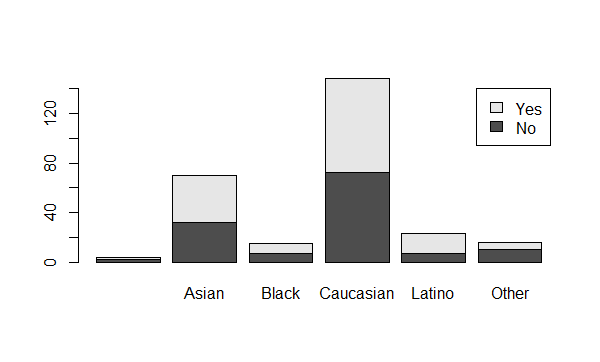
\includegraphics[width=0.7\linewidth]{segmented_barchart}
		\caption{Segmented barchart của DecisionMale và RaceF}
		\label{fig:barchart}
	\end{figure}
	
	Giả sử, ta cần khảo sát sự liên kết giữa dân tộc nữ và sự phản hồi (Yes/No) của nam cho quần thể (population). Từ tổng thể, ta thu thập được một mẫu dữ liệu ngẫu nhiên (random sample) gồm 276 quan sát.
	
	Dựa vào mẫu dữ liệu này, ta kiểm định nghi vấn "Giữa RaceF và DecisionMale có mỗi liên kết với nhau" với mức ý nghĩa (significance level) 5\%.\\
	
	Ta thực hiện kiểm định giả thuyết:
	
	\begin{equation*}
	\begin{cases}
	H_0: & \text{RaceF và DecisionMale độc lập nhau}\\
	H_1: & \text{RaceF và DecisionMale có sự liên kết với nhau}
	\end{cases}
	\end{equation*}
	
	với mức ý nghĩa $\alpha = 0.5\%$\\
	
	\textbf{Trực quan hóa bảng tần suất (2-way frequency table)}
	
	\begin{lstlisting}[language=R]
	> # Load data
	> data <- data.frame(DecisionMale, RaceF)
	> # Significant level
	> alpha <- 0.05
	> 
	> # Frequency table
	> t <- table(data); t
	RaceF
	DecisionMale    Asian Black Caucasian Latino Other
	No   2    32     7        72      7    10
	Yes  2    38     8        76     16     6
	> # P(RaceF|DecisionMale)
	> t.prob <- prop.table(t, margin = 1); t.prob
	RaceF
	DecisionMale                 Asian      Black  Caucasian     Latino      Other
	No  0.01538462 0.24615385 0.05384615 0.55384615 0.05384615 0.07692308
	Yes 0.01369863 0.26027397 0.05479452 0.52054795 0.10958904 0.04109589
	
	> library("graphics")
	> # shade: color graph
	> # las = 1: horizontal labels
	> mosaicplot(t(t), shade = TRUE, las = 1, main = "data")
	\end{lstlisting}
	\footnote{mosaicplot() là hàm built-in của R package \colorbox{green}{graphics}}
	
	\begin{figure}[H]
		\centering
		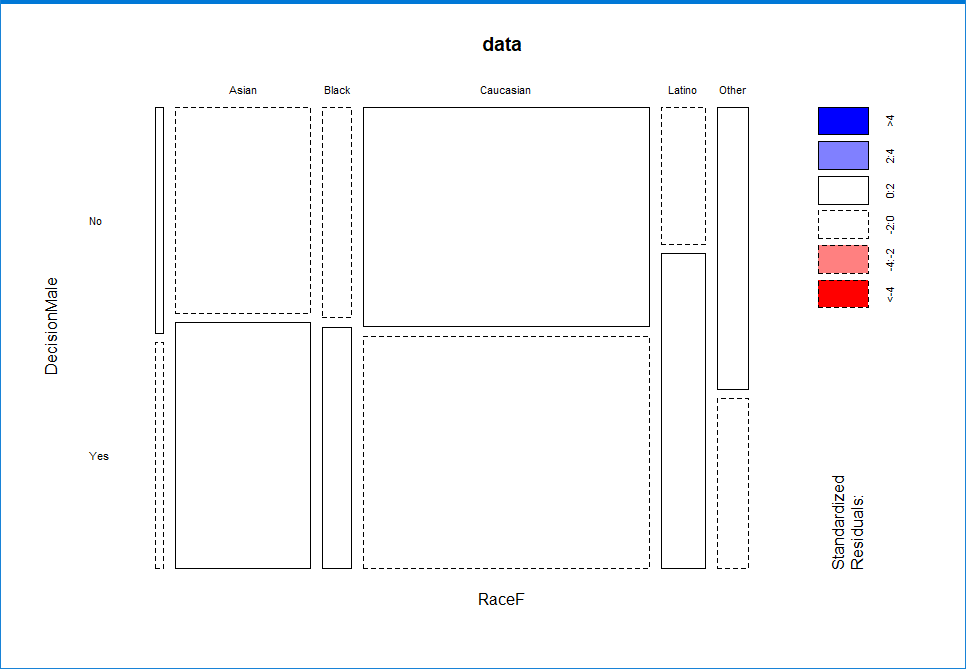
\includegraphics[width=1.0\linewidth]{barchart}
		\caption{Màu đỏ biểu thị observed values bé hơn expected values\\ Màu xanh biểu thị observed values lớn hơn expected values\\ (với điều kiện dữ liệu phải là ngẫu nhiên)}
		\label{fig:barchart}
	\end{figure}
	
	\textbf{Nhận xét}
	\begin{itemize}
		\item Nhìn vào mosaicplot thì ta thấy rằng bảng dữ liệu của chúng ta thấy rằng sự chênh lệch giữa observed values và expected values rất bé. Một phần nào cho ta thấy được giữa RaceF và DecisionMale hầu như không có liên kết.
		
		\item Các ô (cell) màu trắng nét liền biểu thị độ lệch dương và màu trắng nét đứt biểu thị độ lệch âm nhưng ta thầy rằng các độ lệch này rất bé.
	\end{itemize}
	
	Với mỗi ô thì ta có thể tính được expected value tương ứng:
	$$e = \frac{row.sum \ast col.sum}{grand.total}$$
	
	Chi-square statistic tính như sau:
	$$\mathcal{X}^2 = \sum \frac{{(o - e)}^2}{e}$$
	
	với $\begin{cases}
		& \text{o: observed value}\\
		& \text{e: expected value}
	\end{cases}$\\
	
	\textbf{Tính Chi-square statistic trong R}
	
	\begin{lstlisting}[language = R]
	> # Chisq test
	> res <- chisq.test(t); res
	Warning message:
	In chisq.test(t) : Chi-squared approximation may be incorrect
	
	Pearson Chi-squared test
	
	data:  t
	X-squared = 4.2977, df = 5, p-value = 0.5074
	
	> # If p.value < alpha, we ignore H0
	> (res$p.value < alpha)
	[1] FALSE
	
	> # Observed values
	> res$observed
	RaceF
	DecisionMale    Asian Black Caucasian Latino Other
	No   2    32     7        72      7    10
	Yes  2    38     8        76     16     6
	> # Expected values
	> round(res$expected, 2)
	RaceF
	DecisionMale      Asian Black Caucasian Latino Other
	No  1.88 32.97  7.07     69.71  10.83  7.54
	Yes 2.12 37.03  7.93     78.29  12.17  8.46
	\end{lstlisting}
	
	Vì $p-value > \alpha$ nên ta không bác bỏ $H_0$. Như vậy, với mức ý nghĩa 5\%, ta không có đủ căn cứ để bác bỏ "RaceF và DecisionMale độc lập hay nói cách khác cả hai không có sự liên kết".\\
		
	Nhìn vào observed values table và expected values table, ta thấy được rằng chênh lệch ở đây rất ít.
	
	Để biết rõ về bản chất của sự phụ thuộc giữa 2 biến RaceF và DecisionMale, ta sẽ tiếp tục tính dư lượng chuẩn hóa (Standardized residuals hoặc Pearson residuals) cho từng ô để biết được ô nào đóng góp nhiều vào Chi-square $\mathcal{X}^2$:
	$$r = \frac{{o - e}}{\sqrt{e}}$$
	
	Pearson residuals được lấy từ kết quả của chisq.test():
	\begin{lstlisting}[language=R]
	> # Pearson Residuals: Do lech giua observed values and expected values
	> round(res$residuals, 3)
	RaceF
	DecisionMale         Asian  Black Caucasian Latino  Other
	No   0.084 -0.169 -0.025     0.274 -1.165  0.897
	Yes -0.080  0.160  0.023    -0.259  1.099 -0.847
	
	> # Visualize Pearson residuals
	> library(corrplot)
	corrplot 0.84 loaded
	Warning message:
	package ‘corrplot’ was built under R version 3.5.3 
	> corrplot(res$residuals, is.cor = FALSE)
	\end{lstlisting}
	
	\begin{figure}[H]
		\centering
		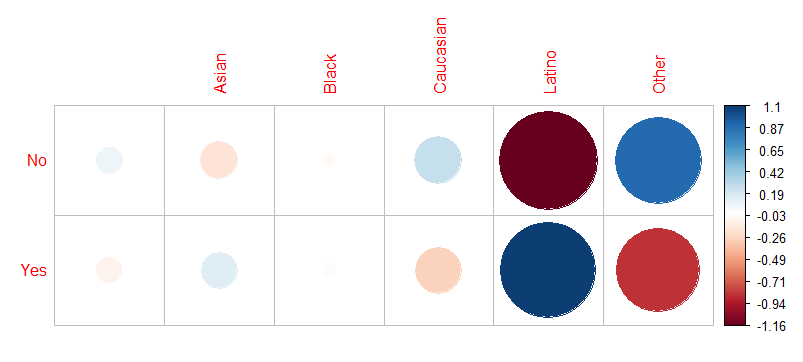
\includegraphics[width=0.7\linewidth]{corplot}
		\caption{Correlation plot}
		\label{fig:corplot}
	\end{figure}
	
	\textbf{Chú thích:}
	\begin{itemize}
		\item Kích thước của hình tròn là tỉ lệ thuận với mức độ đóng góp của ô đó.
		\item Hệ số tương quan ở đây khác với của 2 biến định lượng là không có dao động trong miền [-1, 1]	
	\end{itemize}
	
	
	\textbf{Nhận xét:}
	\begin{itemize}
		\item Màu đỏ biểu thị mối liên kết âm (negative association). Như ta thấy, hàng No và cột Lattino; hàng Yes và các cột Other, Caucasian có mối liên kết âm (negative association) - nghĩa là khi cái này tăng thì cái kia giảm. Ngụ ý là sự không thích (repulsion) , ta có thể thấy dân tộc Latino là nhận nhiều phản hồi No nhất (tức là bị từ chối) và ngược lại, dân tộc Other và Caucasian lại nhận liên kết âm với phản hồi Yes.
		\item Ngược lại, màu xanh biểu thị mối liên kết dương (positive association) - nghĩa là cả hai đều cùng tăng. Như ta thấy, hàng Yes và cột Latino; hàng No và cột Other và Caucasian có liên kết dương. Ngụ ý là sự thu hút (attraction). Điều đó cho thầy người Latino có xu hướng nhận được phản hồi Yes cao. Tương tự, hàng No, cột Other và Caucasian có liên kết dương mạnh, có thể hiểu đơn giản là khi số lượng dân tộc Other và Caucasian tăng thì khả năng họ nhận được phản No (bị từ chối) cũng tăng theo.
	\end{itemize}
	
	Bây giờ, để biết được được mức độ phần trăm đóng góp của các ô cho Chi-square $\mathcal{X}^2$, ta tính theo công thức sau:
	$$contrib = \frac{r^2}{\mathcal{X}^2}$$
	
	\begin{lstlisting}[language=R]
	> # Contribution (Percentage %) of given cell to total chi-squre
	> contrib <- 100*res$residuals^2 / res$statistic
	> round(contrib, 3)
	RaceF
	DecisionMale         Asian  Black Caucasian Latino  Other
	No   0.166  0.665  0.014     1.750 31.561 18.742
	Yes  0.148  0.592  0.012     1.558 28.102 16.688
	
	> # Visualiza contribution
	> corrplot(contrib, is.cor = FALSE)
	\end{lstlisting}
	
	\begin{figure}[H]
		\centering
		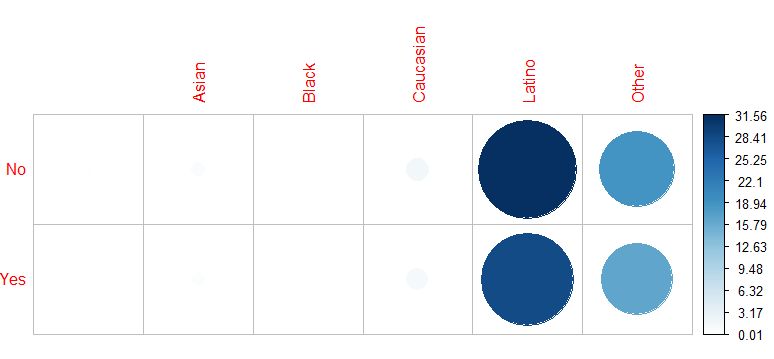
\includegraphics[width=0.7\linewidth]{contrib}
		\caption{Contribution in percentage (\%) plot}
		\label{fig:contrib}
	\end{figure}
	
	Sự đóng góp tương đối của mỗi ô vào tổng Chi bình phương cho thấy một số dấu hiệu về bản chất của sự phụ thuộc giữa các hàng và cột của bảng tần suất.\\
	
	Từ ảnh trên, ta kết luận được:
	\begin{itemize}
		\item Hàng "No" có liên kết mạnh với cột Latino và Other
		\item Hàng "Yes" cũng có liên kết mạnh với Latino và Other
		\item Từ bảng trên tính bằng R, ta thấy các ô đóng góp nhiều cho Chi-squre là No/Latino (31.561\%), No/Other (18.742\%), Yes/Latino (28.102\%) và Yes/Other (16.688\%).
		\item Tổng cộng 4 ô trên đóng góp tới tận 95.048\% vào tổng Chi bình phương và vì vậy chúng chiếm phần lớn sự khác biệt giữa các giá trị kì vọng và giá trị quan sát.
	\end{itemize}
	
	\begin{thebibliography}{00}
		\bibitem{b1} Randall Pruim and Lana Park. Lock5WithR. Chapter 7: Chi-Squared Tests for Categorical Variables. PDF.
		\bibitem{b2} R Users Guide. Chapter 7: Chi-Squared Tests for Categorical Variables. PDF.
		\bibitem{b3} Chi-Square Test of Independence in R. (n.d.). Retrieved from http://www.sthda.com/english/wiki/chi-square-test-of-independence-in-r
		\bibitem{b4} Chi-square Goodness of Fit Test in R. (n.d.). Retrieved from http://www.sthda.com/english/wiki/chi-square-goodness-of-fit-test-in-r
	\end{thebibliography}
\end{document}